\documentclass[slovene,11pt,a4paper]{article}

\usepackage[margin=1.5cm,bottom=3cm,foot=1.5cm]{geometry}
\usepackage{amsmath}
\usepackage{booktabs}
\usepackage{float}
\usepackage{graphicx}
\usepackage{changepage}
\usepackage{subcaption}
\usepackage{multirow}
\usepackage{blindtext}
\usepackage{hyperref}
\usepackage[version=4]{mhchem}
\usepackage[slovene]{babel}


\pagenumbering{gobble}

\begin{document}

\title{2. naloga \\ Klasifikacija zvezdnih spektrov}
\author{Tadej Lozej 28242023}
\maketitle

\begin{center}
Praktikum strojnega učenja v fiziki \\
\bigskip
Predavatelj: red. prof. dr. Borut Paul Kerševan \\
Asistent: doc. dr. Gregor Traven
\end{center}

\newpage

\tableofcontents

\newpage

\pagenumbering{arabic}

\section{Uvod}

V nalogi smo se ukvarjali s spektri zvezd v vidni svetlobi. Spekter je graf jakosti svetlobe pri določeni valovni dolžini. Envelopo spektra zvezde opišemo s Planckovim zakonom. Ta pravi, da vroča telesa sevajo več svetlobe (Štefanov zakon) ter imajo vrh spektra pri manjših valovnih dolžinah. Hladnejša telesa pa ravno obratno. V nalogi smo analizirali normalizirane spektre. To so spektri deljeni z njihovo ovojnico. Zanimale so nas predvsem spektralne črte. Iz njihove oblike namreč lahko izluščimo precej informacij o zvezdi. Na obliko spektralnih črt vpliva veliko fizikalnih procesov/lastnisto zvezde:

\begin{itemize}
    \item \textbf{Temperatura}. Absorpcijske črte se zaradi termičnega gibanja atomov razširijo. Je glavni faktor za obliko spektralnih črt.đ
    \item \textbf{Kovinskost}. Številsko razmerje kovin (elementov težjih od helija) napram vodiku, logaritmirano in normirano na vrednost za Sonce. Kovinskost vpliva na moč posameznih spektralnih črt.
    \item \textbf{Gravitacijski pospešek}. Vpliva na tlačno razširitev črt.
    \item \textbf{Radialna hitrost}. Pove nam kako hitro se zvezda giblje proti ali stran od nas. Ne vpliva na obliko spektralnih črt temveč jih premakne zaradi Dopplerjevega pojava.
    \item \textbf{Rotacijska hitrost}. Zaradi Dopplerjevega pojava razširi črte v polkrožni obliki.
    \item \textbf{Plini okrog zvezde}. Če so ti plini segreti bolj kot površje zvezde lahko sevajo močne emisijske črte.
    \item \textbf{Dvojne zvezde}. To so sistemi, kjer dve zvezde krožita ena okoli druge. Zvezd je v sistemu lahko tudi več. Zaradi Dopplerjevega pojava dobimo podvajanje črt.
\end{itemize}
To je zgolj nekaj fizikalnih lastnosti zvezde, ki vplivajo na spekter zvezde. Poleg vsega tega pa moramo upoštevati še Zemljino atmosfero ter inštrumentalne napake. Na sliki \ref{fig:ucni_spektri} lahko vidimo sedem različnih tipičlnih primerov spektrov. 

\begin{figure}
    \centering
    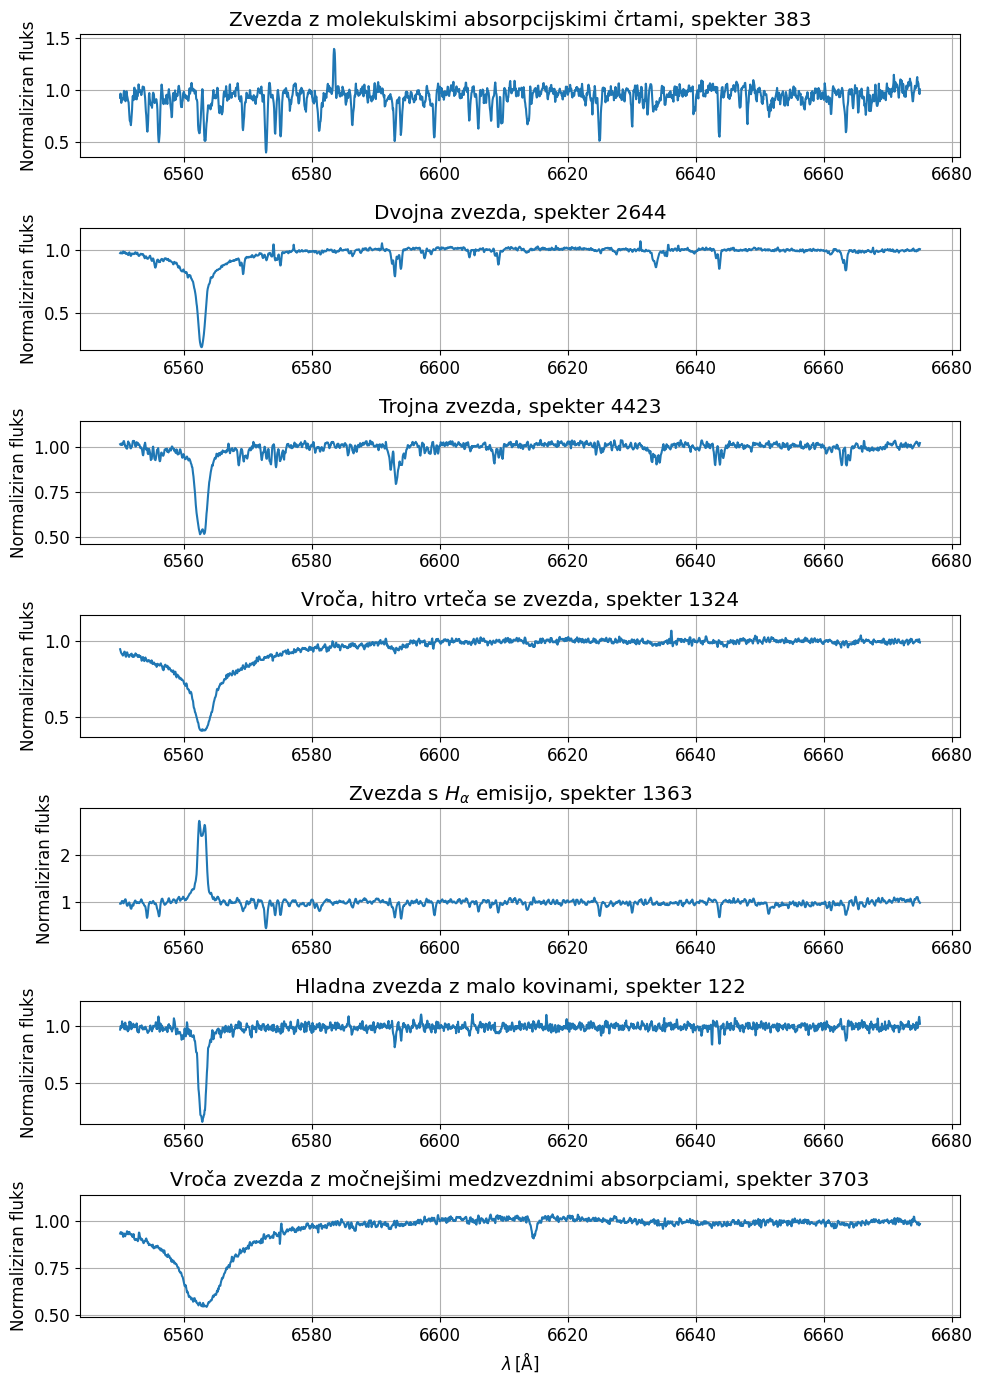
\includegraphics[width=0.95\linewidth]{imgs/ucni_spektri.png}
    \caption{Na sliki je prikazanih 7 normaliziranih spektrov, ki pripadajo različnim tipom zvezd (naslov grafa).}
    \label{fig:ucni_spektri}
\end{figure}

V nalogi imamo na voljo 10000 normaliziranih spektrov zvezd. Za nekaj izmed teh spektrov imamo podane fizikalne lastnosti zvezde. Efektivno temperaturo ($T_{eff}$), logaritem gravitacijskega pospeška ($\log g$) ter kovinskost ($[M/H]$). Za naj spektrov imamo podan tudi tip zvezde. Tipi so prikazani na sliki \ref{fig:ucni_spektri}. V nalogi uporabimo kratice za tip zvezde

\begin{itemize}
    \item \texttt{MAB}: zvezda z molekulskimi absorpcijskimi črtami
    \item \texttt{BIN}: dvojne zvezde
    \item \texttt{TRI}: trojne zvezde
    \item \texttt{HFR}: vroče, hitrovrteče se zvezde
    \item \texttt{HAE}: zvezde s $\text{H}_\alpha$ emisijo
    \item \texttt{CMP}: hladne zvezde z malo kovinami
    \item \texttt{DIB}: vroče zvezde z močnejšimi medzvezdnimi absorpcijami
\end{itemize}

Računsko modeliranje spektrov je zelo zahtevna naloga, zato se v praksi poslužujemo metod strojnega učenja, ki nam spektre pomagajo klasificirati. V tej nalogi si ogledamo dve klasifikacijski metodi, in sicer principal component analysis (PCA) ter t-distributed stochastic neighbor embedding (t-SNE). Obe metodi temeljita na zmanjševanju dimenzij. Vsak spekter v nalogi je opisan s 2084 spremenljivkami. Z temi metodami pa lahko spekter opišemo z recimo dvemi pametno izbranimi dimenzijami, za kateri upamo, da bosta zadovoljivo ločila tipe spektrov med seboj. PCA je linearna metoda, t-SNE je pa bolj napredna nelinearna metoda.

\section{PCA}

Metoda glavnih komponent je ena od osnovnih metod zmanjševanja dimenzij. Je linearna metoda. S to metodo naredimo dekompozicijo našega podatkovnega seta v lastne vektorje in lastne vrednosti. Dimenzije dobljenih lastnih vektorjev so linearna kombinacija vhodnih dimenzij. Lastne vektorje lahko sortiramo od najbolj do najmanj pomembnih po njihovih lastnih vrednostih, ki podajajo varianco podatkov v večdimenzionalnem prostoru. Cilj PCA je poiskati nekaj prvih lastnih vektorjev, ki najbolje opišejo večji del razpršenosti podatkovnega seta. Moja implementacija PCA-ja se nahaja v razdelku Dodatek.

Za začetek si na sliki \ref{fig:lastne_vrednosti} oglejmo normalizirano kumulativno vsoto lastnih vrednosti (modra) ter lastne vrednosti glavnih komponent (rdeča) v logaritemski skali. Vidimo, da je naša PCA metoda našla 2084 novih koordinat, ki jih opisujejo lastni vektorji in jih zložila po padajoči lastni vrednosti. Z nekaj prvimi koordinatami lahko zajamemo večino informacije oz. variance našega podatkovnega seta. Odličimo se za ohranitev 90\% variance. V tem primeru vsak spekter opišemo zgolj z 101 koordinatami. Na grafu lahko vidimo tudi da le prve tri glavne komponente opišejo več kot 70\% raztrešenosti.

\begin{figure}[h!]
    \centering
    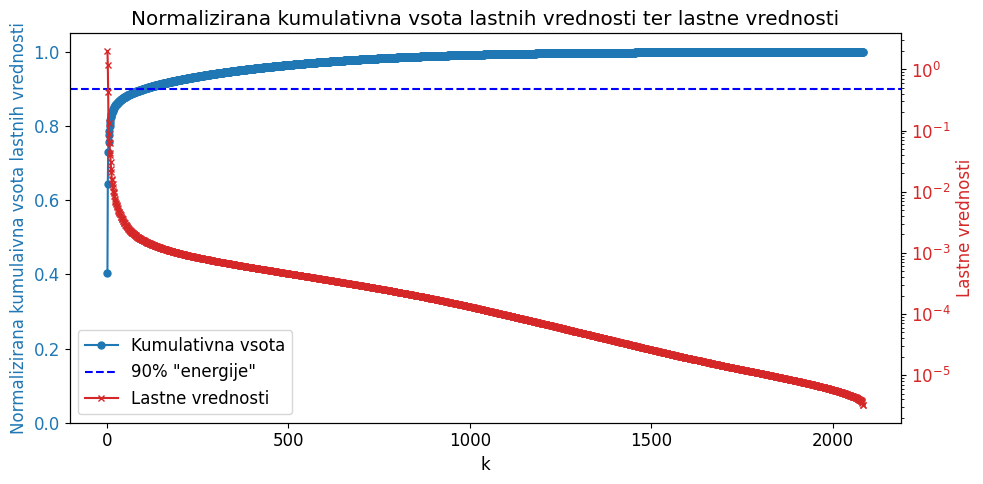
\includegraphics[width=0.95\linewidth]{imgs/lastne_vrednosti.png}
    \caption{Na grafu je prikazana normirana kumulativna vsota lastnih vrednosti (modra) ter lastne vrednosti (rdeča), ki jih dobimo z danim setom podatkov ter PCA metodo. Devetdeset odstotkov variance dosežemo že z zgolj 101 PCA koordinatami.}
    \label{fig:lastne_vrednosti}
\end{figure}

Dvodimenzionalna porazdelitev spektrov s prvimi tremi glavnimi koordinatami je prikazana na sliki \ref{fig:PCA1}. Na $x$ in $y$ oseh so prve tri glavne koordinate PCA metode označene z $PCA_i$. Diagonalni grafi so zgolj histogrami, ki prikazujejo porazdelitev spektrov po glavnih koordinatah. Izvendiagonalni grafi pa prikazujejo dvodimenzionalne porazdelitve po dveh glavnih komponentah.

Na spodnji diagonali lahko vidimo z zvezdicami različnih barv narisane spektre znanega tipa. Vidimo, da metoda ne deluje tako slabo. Vidimo, da so si \texttt{DIB} zvezde precej blizu v vseh porazdelitvah. Enako lahko rečemo za \texttt{TRI} in \texttt{BIN} zvezde. Se pa te dve skupini držita precej skupaj. \texttt{CMP} zvezde se prav tako držijo precej skupaj. Tudi \texttt{HFR} zvezde niso preveč raztrešene. Zelo presenetljivo so precej raztrešene zvezde z $\text{H}_\alpha$ emisijo (\texttt{HAE}). Tega nisem pričakoval, saj imajo precej unikatno značilnost. Zvezde z molekulskimi absorpcijskimi črtami (\texttt{MAB}) so prav tako precej raztrešene v naši porazdelitvi. Zadnja dva rezultata sta me presenetila, saj sta to na videz najbolj očitni lastnosti spektra teh zvezd. Mogoče pa zvezde teh tipov tvorijo več skupkov vendar jih z tako malo znanimi spektri težko ločimo. Kot kaže glavne tri komponente PCA metode precej dobro klasificirajo spektre glede na obliko spektralnih črt.

Na zgornji diagonali lahko vidimo z barvnim gradientom prikazane znane efektivne temperature zvezd. Te so prikazane tudi na histogramskih porazdelitvah. Vidimo lahko, da prva PCA koordinata zelo dobro razvrsti zvezde glede na njihovo efektivno temperaturo.

\begin{figure}[h!]
    \centering
    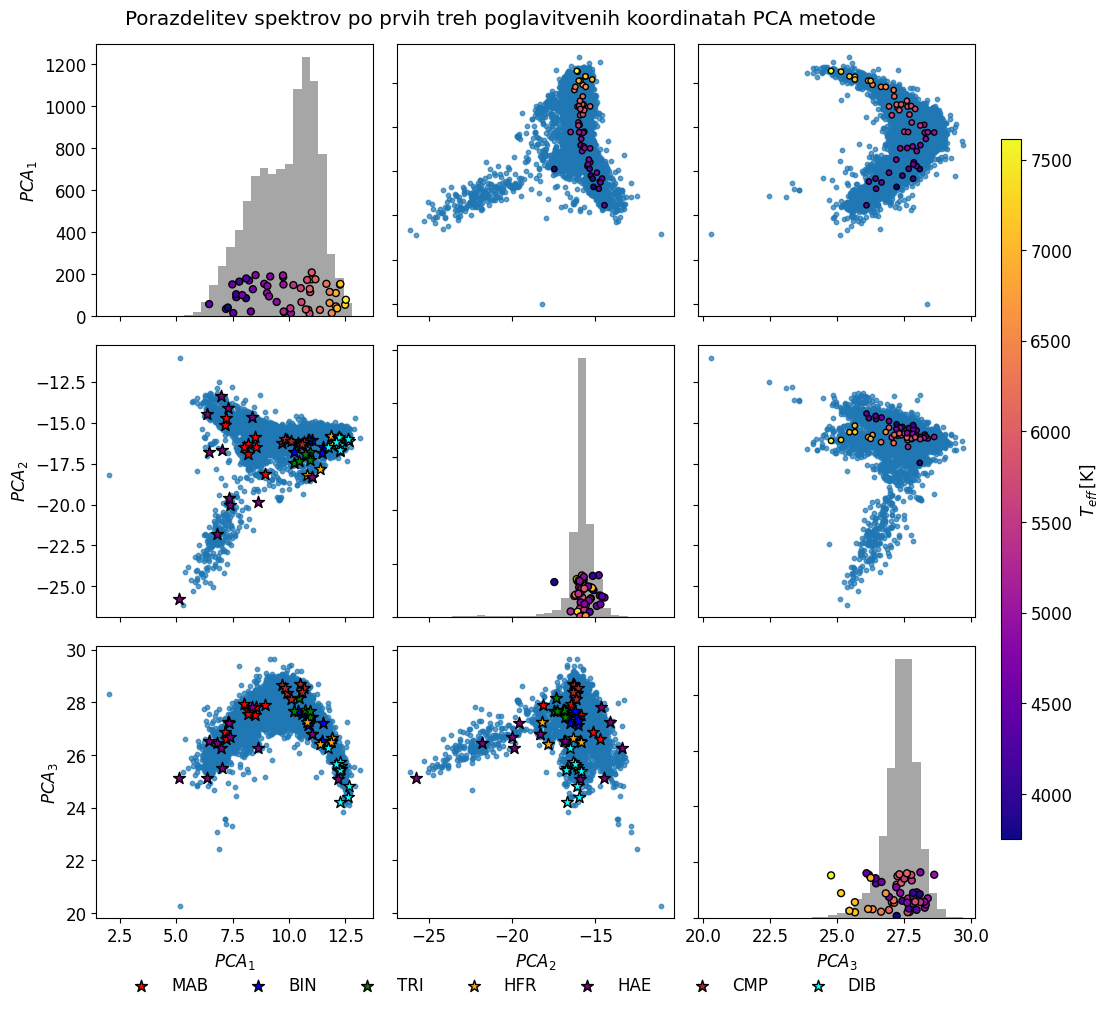
\includegraphics[width=0.95\linewidth]{imgs/PCA1.png}
    \caption{Diagonalni grafi prikazujejo porazdelitev spektrov po prvih treh glavnih PCA koordinatah. Izvendiagonalni grafi prikazujejo dvodimenzionalne porazdelitve spektrov po dveh izmed prvih treh glavnih PCA koordinatah. Na spodnji diagonali so z zvezdami različnih barv prikazani tudi različni tipi spektrov. Na zgornji diagonali ter spodnjem delu histogramov so z barvnim gradientom prikazane znane efektivne temperature zvezd.}
    \label{fig:PCA1}
\end{figure}

Slika \ref{fig:PCA2} je pravzaprav nadaljevanje analize iz prejšnje slike a za drugi dve pomembni fizikalni lastnosti. Enako kot prej vidimo na diagonalnih grafih histograme ter na izvendiagonalnih grafih dvodimenzionalne porazdelitve po prvih treh glavnih PCA koordinatah.

Na spodnji diagonali so z barvnim gradientom poudarjeni znani gravitacijski pospeški zvezd. Prav tako so prikazani tudi na spodnjem delu histogramov. Spet vidimo, da prva glavna PCA koordinata zelo dobro loči spektre glede na gravitacijski pospešek zvezde. Druga in tretja koosrinata ne tako dobro.

Na zgornji diagonali ter na zgornjem delu histogramov lahko z barvnim gradientom vidimo znane vrednosti kovinskosti zvezd. Na prvi pogled nobena izmed prvih treh koordinat ne dobro razloči kovinskosti med seboj.

\begin{figure}[h!]
    \centering
    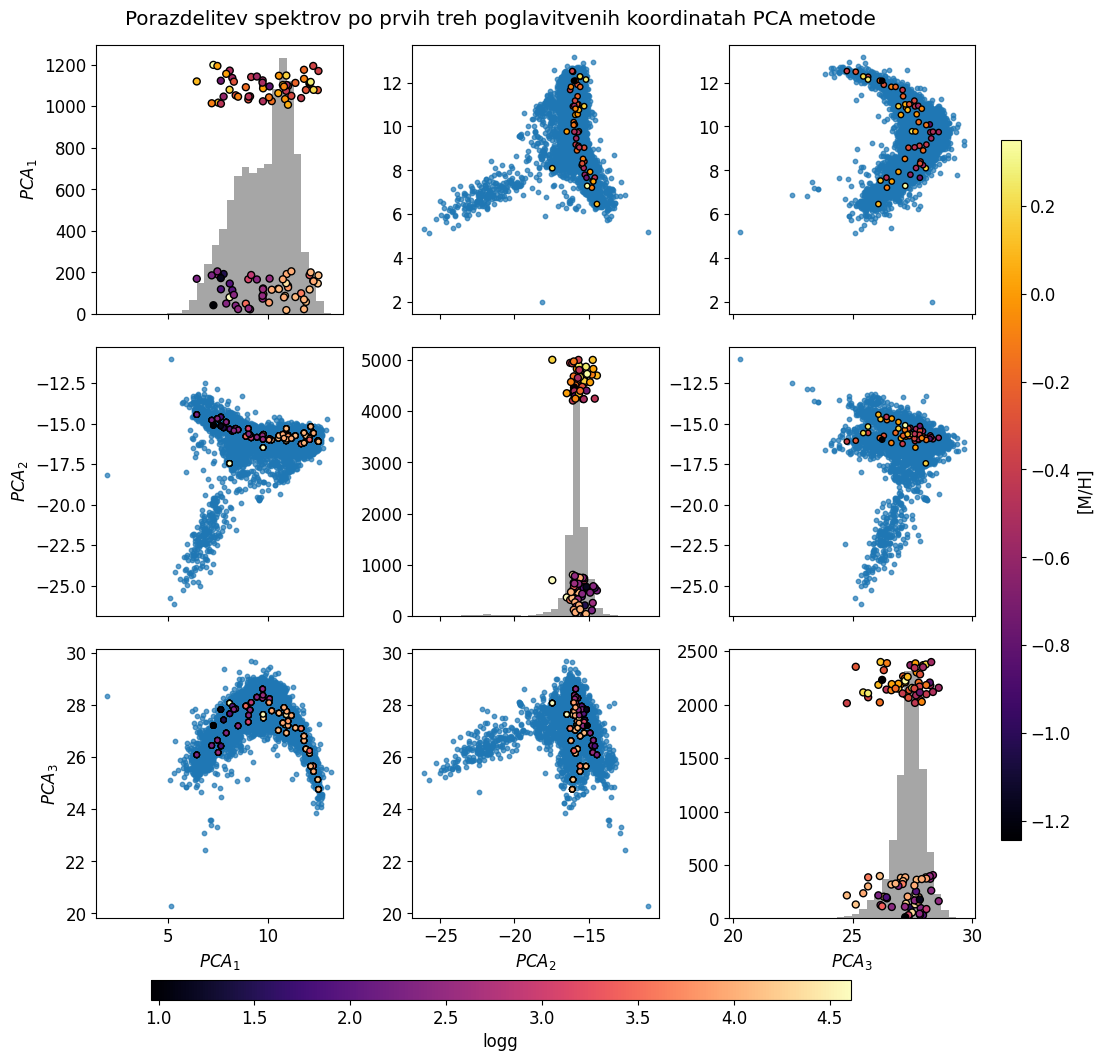
\includegraphics[width=0.95\linewidth]{imgs/PCA2.png}
    \caption{Diagonalni grafi prikazujejo porazdelitev spektrov po prvih treh glavnih PCA koordinatah. Izvendiagonalni grafi prikazujejo dvodimenzionalne porazdelitve spektrov po dveh izmed prvih treh glavnih PCA koordinatah. Na spodnji diagonali ter spodnjem delu histogramov so z barvnim gradientom prikazane znani gravitacijski pospeški zvezd. Na zgornji diagonali ter zgornjem delu histogramov so z barvnim gradientom prikazane znane kovinskosti zvezd.}
    \label{fig:PCA2}
\end{figure}

Med to očesno analizo sem razmišljal o bolj kvantitativnem načinu o tem kako posamezne koordinate dobro opišejo tri omenjene fizikalne količine. Spomnil sem se na preprosti korelacijski koeficient. Na sliki \ref{fig:korelacije1} lahko vidimo porazdelitev spektrov po treh pomembnih fizikalnih količinah ter prvih treh glavnih PCA koordinat. V okvirčku lahko vidimo tudi izračunano Pearsonovo ($r$) ter Spearmanovo ($\rho_s$)korelacijo. Ker se osredotočano na kategorizacijo spektrov predznak korelacije ni pomemben. Rezultat kaže skoraj popolno korelacijo med temperaturo ter prvo glavno PCA koordinato.. Kaže tudi precej dobre korelacije med gravitacijskim pospeškom zvezde ter prvo ter drugo glavno PCA koordinao ter temperaturo ter tretjo glavno PCA koordinato. Kovinskost ima največjo korelacijo s tretjo glavno PCA koordinato.

\begin{figure}[h!]
    \centering
    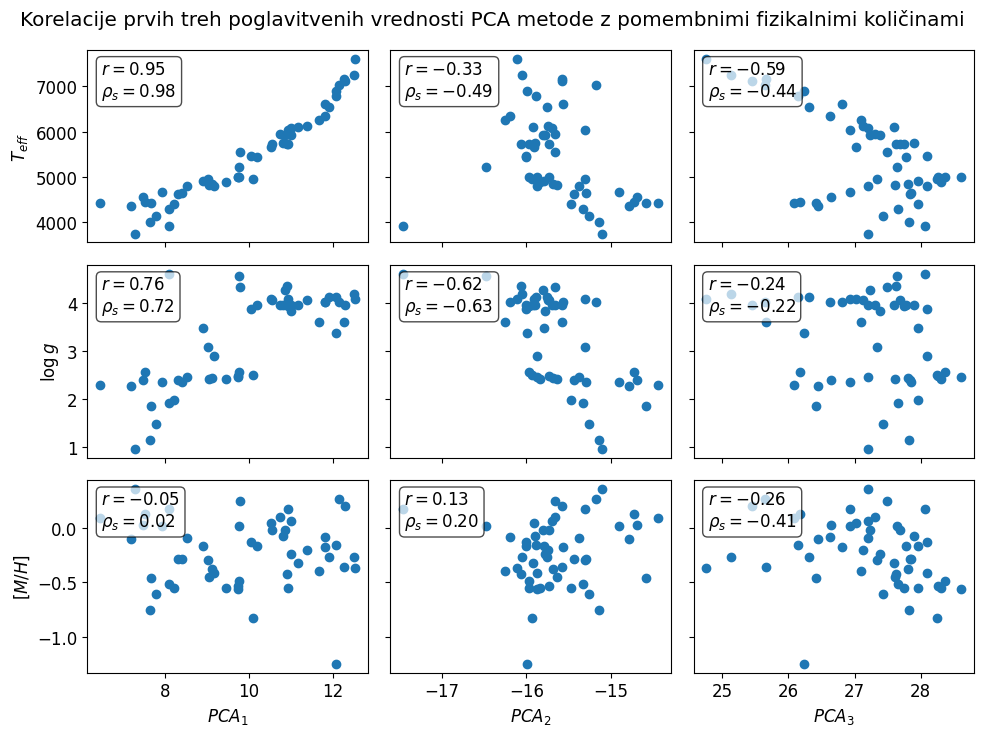
\includegraphics[width=0.95\linewidth]{imgs/korelacije1.png}
    \caption{Porazdelitev spektrov v odvisnosti od treh pomembnih fizikalnih količin ter treh glavnih PCA koordinat. V okvirčkih sta izračunana Pearsonova ter Spearmanova korelacija.}
    \label{fig:korelacije1}
\end{figure}

V upanju, da najdemo boljšo koordinato za opis kovinskosti izračunajmo korelacijo med fizikalnimi količinami ter več PCA koordinatami. Na sliki \ref{fig:korelacije2} lahko vidimo izračunano absolutno Pearsonovo ter Spearmanovo korelacijo med tremi pomembnimi fizikalnimi količinami ter prvimi 101 glavnimi PCA koordinatami. Vidimo, da so korelacije med temperaturo ter prvimi tremi PCA koordinatami največje. Gravitacijski pospešek ima največje korelacije s prvima dvema PCA koordinatama. Tudi v poznejših koordinatah vidimo par večjih korelacij. Kovinskost ima pa največjo korelacijo z sedmo PCA koordinato. Z nobeno koordinato nima tako velike korelacije kot jih imata temperatura ter gravitacijski pospešek.

\begin{figure}[h!]
    \centering
    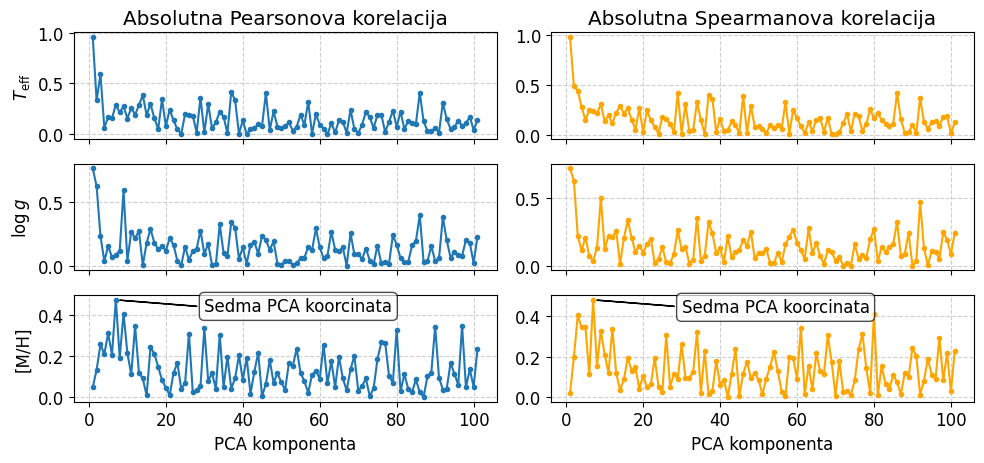
\includegraphics[width=0.95\linewidth]{imgs/korelacije2.png}
    \caption{PEarsonov in Spearmanov korelacijski koeficient med tremi pomembnimi fizikalnimi količinami ter 101 glavnimi PCA koordinatami.}
    \label{fig:korelacije2}
\end{figure}

S tem novim znanejem narišimo še dvodimenzionalno porazdelitev spektrov v odvisnosti od tretje ter sedme PCA koordinate. To lahko vidimo na grafu zgoraj desno na sliki \ref{fig:PCA3}. Opazimo tudi precej manjšo varianco sedme koordinate. Opazimo nek trend naraščajoče kovinskosti vendar niti približno ne tako dober kot s temperaturo ali gravitacijskim pospeškom. Na diagonalnih grafih lahko vidimo porazdelitev spektrov le po tretji ter sedmi koordinati. Na grafu levo spodaj lahko vidimo porazdelitev spektrov po kovinskosti ter sedmi PCA koordinati. V okvirčku vidimo tudi izračunana korelacijska koeficienta.

\begin{figure}[h!]
    \centering
    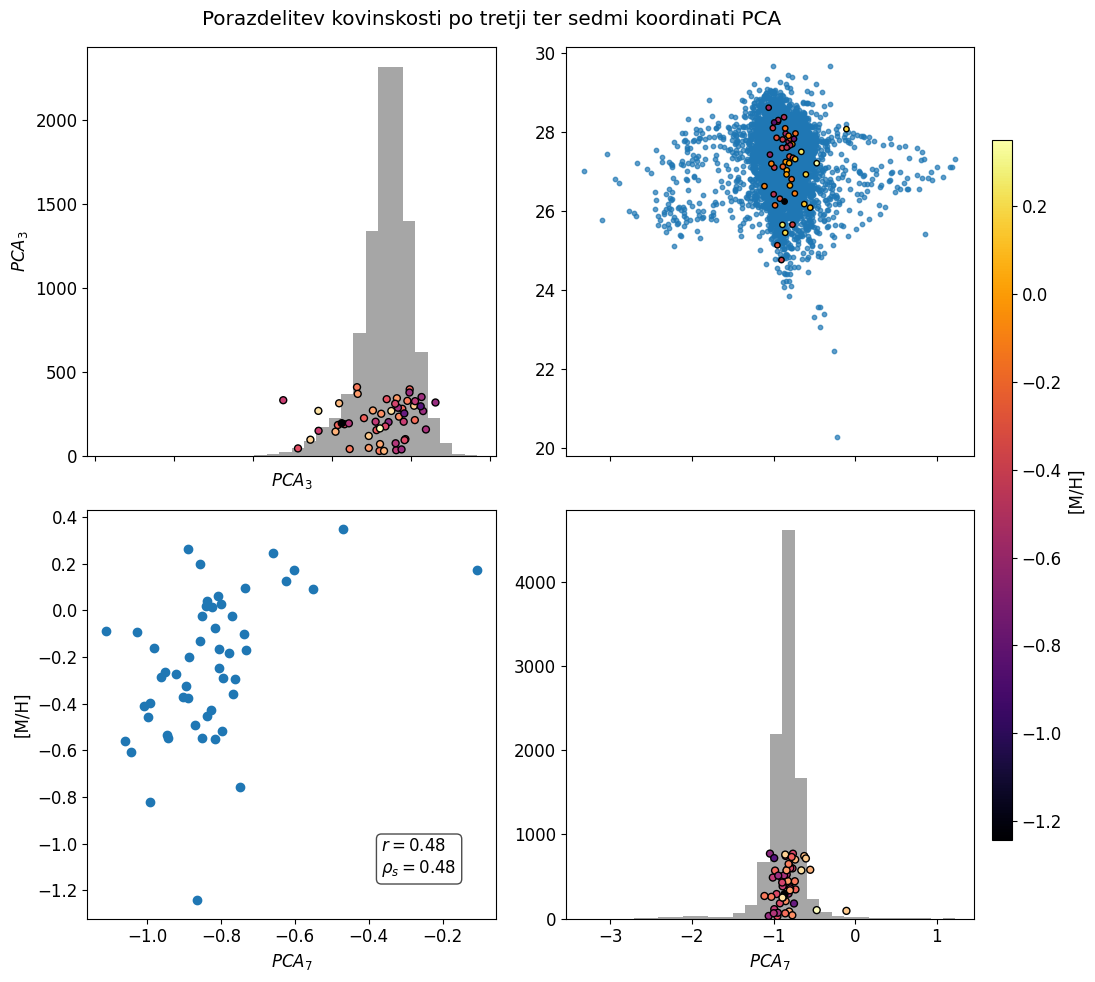
\includegraphics[width=0.95\linewidth]{imgs/PCA3.png}
    \caption{Diagonalna grafa prikazujeta porazdelitev spektrov po tretji ter sedmi PCA koordinati. Zgoraj desno je prikazana dvodimenzionalna porazdelitev spektrov po tretji ter sedmi PCA koordinati. Spodaj levo je prikazana porazdelitev spektrov po kovinskosti ter sedmi PCA koordinati. V okvirčku sta podana tudi Pearsonov ter Spearmanov korelacijski koeficient.}
    \label{fig:PCA3}
\end{figure}

\section{t-SNE}

\newpage

\section{Dodatek}

\begin{figure}[h!]
    \centering
    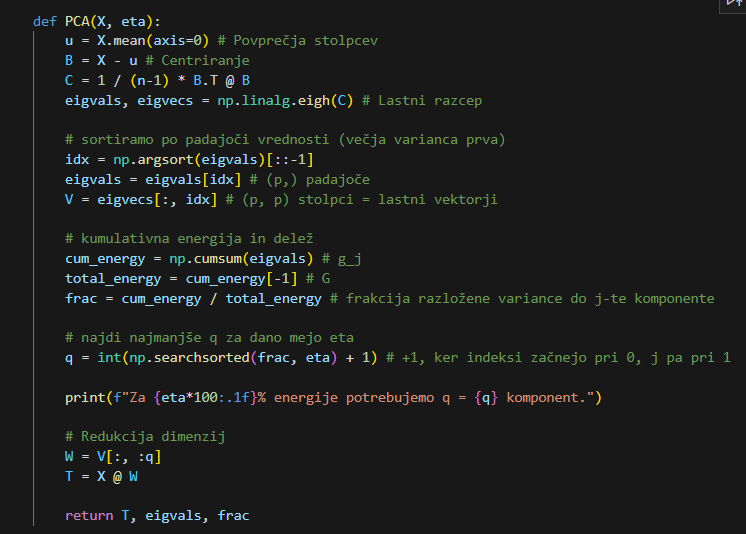
\includegraphics[width=0.95\linewidth]{imgs/koda.png}
    \caption{Python funkcija, ki izvede PCA.}
    \label{fig:koda}
\end{figure}

\end{document}
